% =========================================================================== %

\begin{frame}[t,plain]
\titlepage
\end{frame}

% =========================================================================== %

\begin{frame}{Hofstadter}
%
\begin{columns}
\column{.6\linewidth}
\begin{center}
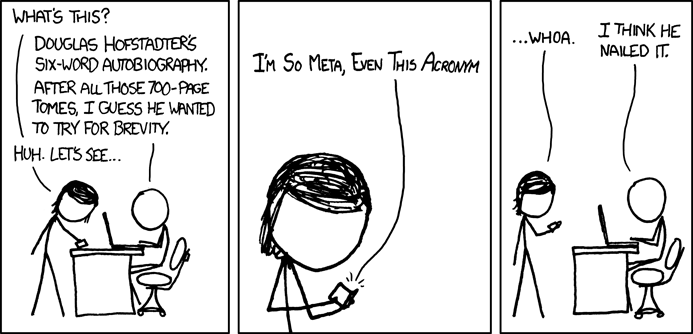
\includegraphics[width=\linewidth]{./gfx/06-xkcd-hofstadter}\\
\end{center}
%
\column{.2\linewidth}
\small
	\emph{\enquote{This is the reference implementation of the self-referential joke.}}

	\vspace{6pt}
	\url{https://xkcd.com/917/}
\end{columns}
%
\end{frame}

% =========================================================================== %

\begin{frame}{Scope For Today}
%
\begin{itemize}
\item Symbol binding
	\begin{itemize}
	\item Reference counting
	\item Lifetime of objects
	\item Mutable and immutable objects
	\item Object dictionaries
	\end{itemize}
\item Self-modifying code
	\begin{itemize}
	\item Concept
	\item Decorators
	\item Examples: runtime decorator and call logger
	\end{itemize}
\item Useful predefined decorators
	\begin{itemize}
	\item \texttt{functools.cache}
	\item \texttt{functools.total\_ordering}
	\item \texttt{functools.partial}
	\end{itemize}
\end{itemize}
%
\end{frame}

% =========================================================================== %

\begin{frame}{Symbol Binding}
%
\begin{itemize}
\item Memory: Long string of one-byte cells
	\begin{itemize}
	\item Enumerated (\enquote{addresses})
	\item Can be grouped into bigger units (\Thus \zB 8 byte per floating point number)
	\item Managed by Python RTS and operating system
	\end{itemize}
\item Code: variable names, aka symbols
	\begin{itemize}
	\item Human readable names for the addresses
	\item Multiple names for same object possible
	\item Multiple contexts (modules, functions, ...)
	\end{itemize}
\item[\Thus] Binding: translation between code symbols (\zB variable names) and memory addresses
	\begin{itemize}
	\item Test with operator \inPy{id}: returns (something like) the address of an object
	\item Objects with same id are the same object in memory
	\item Operator \inPy{is} is equivalent to comparing \inPy{id}s
	\end{itemize}
\end{itemize}
%
\end{frame}

% =========================================================================== %

\begin{frame}[fragile]
%
\begin{tcbraster}[raster columns=2,
                  raster equal height,
                  nobeforeafter,
                  raster column skip=0.2cm]
\begin{codebox}[Equivalent and Equal Objects]
\begin{minted}[linenos, fontsize=\scriptsize]{python3}
A = [1, 2]
B = A
C = [1, 2]

print("id(A) = ", id(A))
print("id(B) = ", id(B))
print("id(C) = ", id(C))
print()

print("A == B:", A == B)
print("A == C:", A == C)
print("B == C:", B == C)
print()

print("A is B:", A is B)
print("A is C:", A is C)
print("B is C:", B is C)
\end{minted}
\end{codebox}
%
\begin{cmdbox}[Output]
\begin{minted}[fontsize=\scriptsize]{text}
id(A) =  140018580051008
id(B) =  140018580051008
id(C) =  140018580049280

A == B: True
A == C: True
B == C: True

A is B: True
A is C: False
B is C: False
\end{minted}
\end{cmdbox}
\end{tcbraster}
%
\end{frame}

% =========================================================================== %

\begin{frame}{Lifetime of Objects and Reference Counting}
%
\begin{itemize}
\item Memory is limited
	\begin{itemize}
	\item[\Thus] Need to re-use memory for our objects
	\item Many languages (like \zB C): manually \emph{allocate} and \emph{deallocate/free} memory
	\item Python
		\begin{itemize}
		\item Automatically (at least by default)
		\item Operator \inPy{del}: manually free ressources (up to a degree)
		\end{itemize}
	\end{itemize}
\item Consequence: Need mechanism to decide when to free object memory
	\begin{itemize}
	\item[\Thus] \emph{Reference counting} and \emph{Garbage collection}
	\item Each object \enquote{knows} how many symbols are bound to it
	\item If reference count drops to zero -- free memory
	\item \texttt{sys.getrefcount} -- gives you exactly that
	\item Result usually one higher than expected -- local variable in \texttt{getrefcount}
	\end{itemize}
\end{itemize}
%
\end{frame}

% =========================================================================== %

\begin{frame}[fragile]
%
\begin{tcbraster}[raster columns=2,
                  raster equal height,
                  nobeforeafter,
                  raster column skip=0.2cm]
\begin{codebox}[Reference Counting]
\begin{minted}[linenos, fontsize=\scriptsize]{python3}
import sys

x = ["some value"]
y = x

print("y is ", 
      "" if y is x else "not ", 
      "x", sep="")
print("refs to object with name x:", 
      sys.getrefcount(x))
print("refs to object with name y:", 
       sys.getrefcount(y))

del x
# no longer possible, gives NameError
# print(x is y)
# print(sys.getrefcount(x))

print("y =", y)
print(sys.getrefcount(y))
\end{minted}
\end{codebox}
%
\begin{cmdbox}[Output]
\begin{minted}[fontsize=\scriptsize]{text}
y is x
refs to object with name x: 3
refs to object with name y: 3
y = ['some value']
2
\end{minted}
\end{cmdbox}
\end{tcbraster}
%
\end{frame}

% =========================================================================== %

\begin{frame}{Extension of Lifetime}
%
\begin{itemize}
\item Symbols can go out of scope
	\begin{itemize}
	\item I.\;e. they exist in a function and code execution leaves the function scope
	\end{itemize}
\item Object behind symbol may live on
	\begin{itemize}
	\item E.\;g. return value of functions
	\item E.\;g. parameter to the function
	\end{itemize}
\item Symbols may be rebound
	\begin{itemize}
	\item Assigning a new object to a symbol
	\item Other references to object not affected
	\end{itemize}
\end{itemize}
%
\begin{hintbox}[Track Object IDs]
\small
It can be a bit nebulous at times when objects actually die and when they live on with different names. In doubt, use the \inPy{is} and \inPy{id} operators to confirm your assumptions. This also helps you find possibly time consuming copy actions!
\end{hintbox}
%
\end{frame}

% =========================================================================== %

\begin{frame}[fragile]
%
\begin{tcbraster}[raster columns=2,
                  raster equal height,
                  nobeforeafter,
                  raster column skip=0.2cm]
\begin{codebox}[Rebinding Objects]
\begin{minted}[linenos, fontsize=\scriptsize]{python3}
def mutating_read_access(data):
    print("### IN MUTATING_READ_ACCESS")
    data.append(1)
    print("data =", data)
    print("id(data) =", id(data))
    data = [2]   # variable is rebound!
    print("after overwriting:")
    print("data =", data)
    print("id(data) =", id(data))
    print()

array = []
print("array =", array)
print("id(array) = ", id(array))
print()

mutating_read_access(array)

print("### ON MODULE LEVEL")
print("array =", array)
\end{minted}
\end{codebox}
%
\begin{cmdbox}[Output: Rebinding Objects]
\begin{minted}[fontsize=\scriptsize]{text}
array = []
id(array) =  140342256155328

### IN MUTATING_READ_ACCESS
data = [1]
id(data) = 140342256155328
after overwriting:
data = [2]
id(data) = 140342256182912

### ON MODULE LEVEL
array = [1]
\end{minted}
\end{cmdbox}
\end{tcbraster}
%
\end{frame}

% =========================================================================== %

\begin{frame}{Mutable and Immutable Objects}
%
\begin{itemize}
\item Python distinguishes between \emph{mutables} and \emph{immutables}
	\begin{itemize}
	\item Values that can be changed and cannot be changed
	\item Immutables can still be created and destroyed
	\item \enquote{Changing} always only rebinds the variable
	\end{itemize}
\item Immutables are ...
	\begin{itemize}
	\item primitive data types: \inPy{bool}s, \inPy{int}s, \inPy{float}s, \inPy{complex}s and \inPy{str}ings
	\item very few containers: \inPy{tuple}s, \inPy{frozenset}s and \inPy{bytes}
	\item some \inPy{import}able objects like \texttt{frozendict}s
	\item functions and modules
	\end{itemize}
\item Mutables are ...
	\begin{itemize}
	\item everything else
	\end{itemize}
\end{itemize}
%
\end{frame}

% =========================================================================== %

\begin{frame}[fragile]{Tangent: Reference Count of Low Valued Integers}
%
\begin{itemize}
\item The line \inPy{sys.getrefcount(1)} will give you a seemingly impossibly high result
	\begin{itemize}
	\item Example when I last tried it: \texttt{864}
	\item Simply loading another module will change the result
	\end{itemize}
\item Reason: \inPy{1} is a \inPy{int} and thus immutable
	\begin{itemize}
	\item If it can't change, it can safely be shared between objects
	\item All the inner workings of Python, \texttt{sys}, \texttt{numpy}, ... share the same \inPy{1}
	\end{itemize}
\item Reason 2: Python pre-allocates often-used objects to save time in the long run
	\begin{columns}
	\column{.4\linewidth}
\begin{minted}[fontsize=\footnotesize]{python3}
a = 1
b = 1
print(a is b)
\end{minted}
		gives \texttt{True}
%	%
	\column{.4\linewidth}
\begin{minted}[fontsize=\footnotesize]{python3}
a = 256
b = 256
print(a is b)
\end{minted}
		gives \texttt{False}
	\end{columns}
\item See \url{https://groverlab.org/hnbfpr/2017-06-22-fun-with-sys-getrefcount.html}
\end{itemize}
%
\end{frame}

% =========================================================================== %

\begin{frame}{Behind the Scenes: \inPy{globals} and \inPy{locals}}
%
\begin{itemize}
\item Command \inPy{globals}
	\begin{itemize}
	\item Creates a \inPy{dict}: \inPy{str} \thus \inPy{object}
	\item Symbol to object
	\item Data is always present, but \inPy{dict} only materializes when calling \inPy{globals}
	\item But: editing the dict really affects RTE
		\begin{itemize}
		\item Allows changing values of existing variables
		\item Allows removing existing variables (like \inPy{del variable})
		\item Allows creation of new variables
		\end{itemize}
	\end{itemize}
\item Command \inPy{locals}
	\begin{itemize}
	\item Same, but for local scope, \ie only within current function
	\end{itemize}
\end{itemize}
%
\begin{hintbox}[Useful for debug]
\footnotesize
The commands \inPy{globals} and \inPy{locals} can be useful for debug -- one line shows the entire state of the program. Code that depends on these commands for its core funcitonality become complex and hard to handle quickly.
\end{hintbox}
%
\end{frame}

% =========================================================================== %

\begin{frame}[fragile]
%
\begin{tcbraster}[raster columns=2,
                  raster equal height,
                  nobeforeafter,
                  raster column skip=0.2cm]
\begin{codebox}[\texttt{globals} and \texttt{locals}]
\begin{minted}[linenos, fontsize=\scriptsize]{python3}
def foo():
    x = 7
    print(locals())
    
x = 1
y = x
print(x is y)

globals()['x'] = 2
globals()['z'] = 3

print(globals())
print(x is y)
print(y)
print(z)

foo()
\end{minted}
\end{codebox}
%
\begin{cmdbox}[Output: \texttt{globals} and \texttt{locals}]
\begin{minted}[fontsize=\scriptsize]{text}
True
{'__name__': '__main__', 
 '__doc__': None, 
 '__package__': None, 
 '__loader__': 
     <class '_frozen_importlib.
             BuiltinImporter'>, 
 '__spec__': None, 
 '__annotations__': {}, 
 '__builtins__':
      <module 'builtins' (built-in)>, 
 'foo': <function foo at 0x7ff7d027e0e0>, 
 'x': 2, 
 'y': 1, 
 'z': 3}
False
1
3
{'x': 7}
\end{minted}
\end{cmdbox}
\end{tcbraster}
%
\end{frame}

% =========================================================================== %

\begin{frame}{Modifying Functions}
%
\begin{itemize}
\item Functions are Python \texttt{object}s, too
	\begin{itemize}
	\item Immutable \Thus we can't \emph{directly} change the code at runtime
	\item Full set of mechanisms, in particular binding of symbol to object and reference counting
	\item Can be return values of functions
	\item Think of operators like $\dv{x}$: They, too, compute a function from a function
	\end{itemize}
\item Symbols can be rebound to other functions
	\begin{itemize}
	\item Original function object is preserved if references continue to exist
	\item Each function has its \inPy{locals()} object
	\item Each \inPy{locals()} object can hold references to functions
	\end{itemize}
\item[\Thus] We can create wrappers around our functions
\end{itemize}
%
\begin{hintbox}[Nomenclature]
Functions that take a function and return a modified function are called \emph{decorators}.
\end{hintbox}
%
\end{frame}

% =========================================================================== %

\begin{frame}[fragile]{Half of an Example}
%
\begin{codebox}[Numerical Derivative Functional]
\begin{minted}[linenos, fontsize=\scriptsize]{python3}
def derivative(f, epsilon = 1E-6):
    def wrapper(x):
        return (f(x + epsilon) - f(x - epsilon)) / (2 * epsilon)
    return wrapper

cosine = derivative(math.sin)
cosine_lores = derivative(math.sin, 1E-2)
print(cosine(0))         # output: 0.9999999999998334
print(cosine_lores(0))   # output: 0.9999833334166665
\end{minted}
\end{codebox}
%
\begin{itemize}
\item \texttt{wrapper} exists in \inPy{locals} of \texttt{derivative}
\item Each call to \texttt{derivative} creates a new set of local variables
\item \texttt{cosine} and \texttt{cosine\_lores} will each hold a reference to one distinct object \texttt{wrapper}
\item The \texttt{wrapper} in turn will hold references to the origninal \texttt{f} and to \texttt{epsilon}
\end{itemize}
%
\end{frame}

% =========================================================================== %

\begin{frame}[fragile]{The Other Half}
%
\begin{codebox}[Modifying Behaviour]
\begin{minted}[linenos, fontsize=\scriptsize]{python3}
def timed(f):
    def wrapper(*args, **kwargs):
        tic = time.perf_counter()
        result = f(*args, **kwargs)
        toc = time.perf_counter()
        return result, toc - tic
    return wrapper

def simulation(...):
    ...

simulation = timed(simulation)
\end{minted}
\end{codebox}
%
\small
\vspace{-6pt}
\begin{itemize}
\setlength{\itemsep}{0pt}
\item Symbol \texttt{simulation} is now tied to code of \texttt{wrapper}
\item The object behind \texttt{wrapper} still holds code of original \texttt{simulation}
\item Calling \texttt{simulation} now returns a \inPy{tuple} of original result and runtime
\end{itemize}
%
\end{frame}

% =========================================================================== %

\begin{frame}[fragile]{A Shortform}
%
\begin{codebox}[Decorator{,} Longform]
\begin{minted}[linenos, fontsize=\scriptsize]{python3}
def decorator(f):
    ...
def function(...):
    ...
function = decorator(function)
\end{minted}
\end{codebox}
%
is equivalent to
\begin{codebox}[Decorator{,} Shortform]
\begin{minted}[linenos, fontsize=\scriptsize]{python3}
def decorator(f):
    ...
@decorator
def function(...):
    ...
\end{minted}
\end{codebox}
%
\end{frame}

% =========================================================================== %

\begin{frame}[fragile]{Notes on Decorators and the Shortform Syntax}
%
\begin{itemize}
\item For the shortform sytnax, the decorator must take exactly one argument:\\
	the object to modify
	\begin{itemize}
	\item Parametrized decorators are only indirectly possible (see next slide)
	\end{itemize}
\item The returned object can be anything
	\begin{itemize}
	\item It \emph{should be} a callable, though
	\item Can be a lambda, a function or a class instance with dunder \inPy{__call__}
	\end{itemize}
\item The decorator must itself be \emph{any} callable
	\begin{itemize}
	\item Can also be a \inPy{class}
	\item The dunder \inPy{__init__} then acts as the decorator
	\end{itemize}
\item Number of arguments of returned object needs not match that of original function
	\begin{itemize}
	\item E.\;g. it is possible to hide parameters or fill in defaults
	\item \texttt{functools.partial} does exactly that
	\end{itemize}
\item There are some meta-properties that naive decorators mess up
	\begin{itemize}
	\item We haven't discussed them yet \Thus another lecture
	\item \texttt{functools.wraps} circumvents this problem
	\end{itemize}
\end{itemize}
%
\end{frame}

% =========================================================================== %

\begin{frame}[fragile]
%
\begin{codebox}[Parametrized decorator]
\begin{minted}[linenos, fontsize=\scriptsize]{python3}
def derivative(epsilon = 1E-6):
    def decorator(f):
        def wrapper(x):
            return (f(x + epsilon) - f(x - epsilon)) / (2 * epsilon)
        return wrapper
    return decorator

@derivative(1E-5)
def f(x):
    return 2*x

print(f(58008))    # output: 2.0000006770715117
\end{minted}
\end{codebox}
%
\begin{hintbox}[Very mature example]
\footnotesize
See \url{https://www.smbc-comics.com/?id=3599} \\
and \url{https://www.urbandictionary.com/define.php?term=58008}
\end{hintbox}
%
\end{frame}

% =========================================================================== %

\begin{frame}[fragile]{A Silly Example}
%
\begin{codebox}[Non-Callable Decoration]
\begin{minted}[linenos, fontsize=\scriptsize]{python3}
def modifier(f):
    return 4

@modifier
def four():
    pass

print(four)   # note: no call!
\end{minted}
\end{codebox}
%
\begin{cmdbox}[Output: Non-Callable Decoration]
\begin{minted}[fontsize=\scriptsize]{text}
4
\end{minted}
\end{cmdbox}
%
\end{frame}

% =========================================================================== %

\begin{frame}[fragile]
%
\begin{codebox}[A Better Example: Callable Class Decorator]
\begin{minted}[linenos, fontsize=\scriptsize]{python3}
class LoggedFunction:
    indent = 0
    delta_indent = 2

    def __init__(self, f):
        self.f = f

    def __call__(self, *args, **kwargs):
        print(" " * self.indent, "calling", self.f.__name__,
              "with arguments", args, kwargs)
        self.indent += self.delta_indent

        result = self.f(*args, **kwargs)

        self.indent -= self.delta_indent
        print(" " * self.indent, "returning from", self.f.__name__,
              "with result", result)
        return result
\end{minted}
\end{codebox}
%
\end{frame}

% =========================================================================== %

\begin{frame}[fragile]
%
\begin{codebox}[Callable Class Decorator Continued]
\begin{minted}[linenos, firstnumber=last, fontsize=\scriptsize]{python3}
@LoggedFunction
def fib(N):
    if N  < 0: return 0
    if N == 0: return 0
    if N == 1: return 1
    return fib(N - 1) + fib(N - 2)

print(fib(3))
\end{minted}
\end{codebox}
%
\begin{hintbox}[Do you see the problem?]
This is the textbook implementation of the algorithm to find the $N^{\text{th}}$ Fibonacci number. It is horribly slow.
\end{hintbox}
%
\end{frame}

% =========================================================================== %

\begin{frame}[fragile]
%
\begin{cmdbox}[Output: Non-Callable Decoration]
\begin{minted}[fontsize=\scriptsize]{text}
 calling fib with arguments (3,) {}
   calling fib with arguments (2,) {}
     calling fib with arguments (1,) {}
     returning from fib with result 1
     calling fib with arguments (0,) {}
     returning from fib with result 0
   returning from fib with result 1
   calling fib with arguments (1,) {}
   returning from fib with result 1
 returning from fib with result 2
2
\end{minted}
\end{cmdbox}
%
\begin{hintbox}[Computing the same values over and over]
As you can see, \texttt{fib(1)} is computed twice (once from the \texttt{fib(N-1)} branch and once from the \texttt{fib(N-2)} branch).
This exponentially accumulates computation overhead!
\end{hintbox}
%
\end{frame}

% =========================================================================== %

\begin{frame}[fragile]{Solution: Caching Results}
%
\begin{itemize}
\item Use a \inPy{dict}: \emph{argument} \thus \emph{previously computed result}
	\begin{itemize}
	\item If \emph{argument} not in \inPy{dict}: proceed normally, but store result in \inPy{dict}
	\item Otherwise: just return value from \inPy{dict}
	\end{itemize}
\item Useful also for non-recursive scenarios
	\begin{itemize}
	\item Anything that takes more time to compute than to look up
	\item and is called somewhat frequently
	\end{itemize}
\item We could implement this ourselves ...
\item ... or use \texttt{functools.cache}
	\begin{itemize}
	\item (in case of class methods: \texttt{functools.cached\_property})
	\end{itemize}
\end{itemize}
%
\end{frame}

% =========================================================================== %

\begin{frame}[fragile]
%
\begin{columns}
\column{.42\linewidth}
\begin{codebox}[Cached Fibonacci, equal height group=cachedFib]
\begin{minted}[linenos, fontsize=\scriptsize]{python3}
@functools.cache
@LoggedFunction
def fib_cached(N):
    if N  < 0: return 0
    if N == 0: return 0
    if N == 1: return 1
    return fib_cached(N - 1) + \
           fib_cached(N - 2)

print("### CACHED FIB")
print(fib_cached(5))

print("### PRECOMPUTED " +
      "INTERMEDIATE RESULT")
print(fib_cached(2))
\end{minted}
\end{codebox}
%
\column{.57\linewidth}
\begin{cmdbox}[Output: Cached Fibonacci, equal height group=cachedFib]
\begin{minted}[fontsize=\scriptsize]{text}
calling fib_cached with arguments (5,) {}
  calling fib_cached with arguments (4,) {}
    calling fib_cached with arguments (3,) {}
      calling fib_cached with arguments (2,) {}
        calling fib_cached with arguments (1,) {}
        returning from fib_cached with result 1
        calling fib_cached with arguments (0,) {}
        returning from fib_cached with result 0
      returning from fib_cached with result 1
    returning from fib_cached with result 2
  returning from fib_cached with result 3
returning from fib_cached with result 5
5

### PRECOMPUTED INTERMEDIATE RESULT
 calling fib_cached with arguments (2,) {}
 returning from fib_cached with result 1
1
\end{minted}
\end{cmdbox}
\end{columns}
%
\end{frame}

% =========================================================================== %

\begin{frame}[fragile]
%
\begin{codebox}[Pseudo-Caching]
\begin{minted}[linenos, fontsize=\scriptsize]{python3}
def fib(N):
    if N  < 0: return 0
    if N == 0: return 0
    if N == 1: return 1
    return fib(N - 1) + fib(N - 2)

simple_fib = timed(fib)
pseudo_cached_fib = timed(functools.cache(fib))

@functools.cache
def fib_cached(N):
    if N  < 0: return 0
    if N == 0: return 0
    if N == 1: return 1
    return fib_cached(N - 1) + fib_cached(N - 2)

correctly_cached_fib = timed(fib_cached)
\end{minted}
\end{codebox}
%
\begin{hintbox}[]
\footnotesize
\texttt{pseudo\_cached\_fib} applies the cache only on the outermost layer, not within computation itself.
\end{hintbox}
%
\end{frame}

% =========================================================================== %

\begin{frame}{Time Complexity}
%
\vspace{-3pt}
\begin{columns}
\column{.45\linewidth}
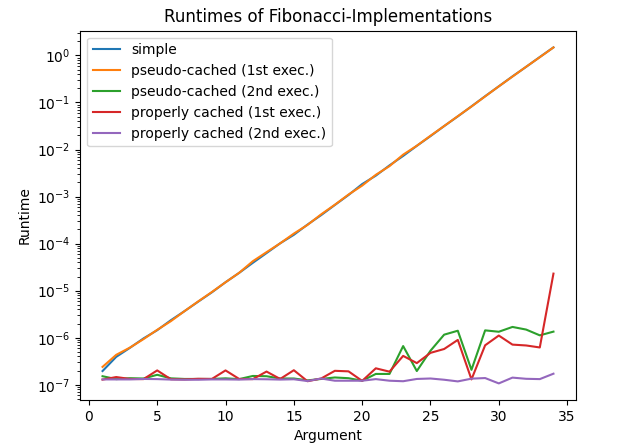
\includegraphics[width=\linewidth]{./gfx/06-cached-fib}
%
\column{.45\linewidth}
\begin{itemize}
\item Uncached: $\mathcal{O}(\exp(N))$
\item Pseudo-Cached: 
	\begin{itemize}
	\item $\mathcal{O}(\exp(N))$ for $1^{\text{st}}$ call
	\item $\mathcal{O}(1)$ for subsequent calls
	\end{itemize}
\item Properly Cached: 
	\begin{itemize}
	\item $\mathcal{O}(N)$ for $1^{\text{st}}$ call
	\item $\mathcal{O}(1)$ for subsequent calls
	\end{itemize}
\end{itemize}
\end{columns}
%
\begin{hintbox}[Going from Exponential to Linear Time Complexity is Huge]
\footnotesize
Assume \texttt{f} has exponential time complexity, and \texttt{f(1)} takes 1 second to compute. Then \texttt{f(18)} takes already longer than the lifetime of the universe.
Compare that to \texttt{g}: linear time complexity, which only takes 18 seconds...
\end{hintbox}
%
\end{frame}

% =========================================================================== %

\begin{frame}{Decorators and Classes}
%
\begin{itemize}
\item Class methods can be decorated, too
	\begin{itemize}
	\item Usually just as with normal functions
	\item When order of parameters relevant: keep the implicit \inPy{self} argument in mind
	\item Example: \texttt{functools.cached\_property}
	\end{itemize}
\item Classes themselves can be decorated
	\begin{itemize}
	\item Decorator then takes argument \inPy{cls} (naming convention)
	\item Represents undecorated class
	\item Process class attributes and methods of undecorated class
	\item Return a \emph{class}
	\item Example: \texttt{functools.total\_ordering}
		\begin{itemize}
		\item Expects compare equal (\inPy{__eq__}) and \emph{one other} compare dunder (\inPy{__lt__}, \inPy{__le__}, \inPy{__gt__} or \inPy{__ge__}) to be present
		\item Synthesizes the rest of them, including (\inPy{__ne__})
		\end{itemize}
	\end{itemize}
\end{itemize}
%
\end{frame}

% =========================================================================== %

\begin{frame}[fragile]
%
\begin{tcbraster}[raster columns=2,
                  raster equal height,
                  nobeforeafter,
                  raster column skip=0.2cm]
\begin{codebox}[Annoy Your Fellow Mathematicians]
\begin{minted}[linenos, fontsize=\scriptsize]{python3}
import functools

@functools.total_ordering
class ordered_complex(complex):
    def __lt__(self, other):
        return abs(self) < abs(other)

z1 = ordered_complex(1, 0)
z2 = ordered_complex(0, 1)
print(z1, z2)
print(z1 < z2)
print(z1 > z2)
print(z1 == z2)
print(z1 != z2)
\end{minted}
\end{codebox}
%
\begin{cmdbox}[Output]
\begin{minted}[fontsize=\scriptsize]{text}
(1+0j) 1j
False
False
False
True
\end{minted}
\end{cmdbox}
\end{tcbraster}
%
\begin{hintbox}[Extra Lazy Example]
\footnotesize
The method \inPy{__eq__} is already implemented in the base class \inPy{complex}.
\end{hintbox}
%
\end{frame}

% =========================================================================== %

\begin{frame}[fragile]{\texttt{functools.partial} -- Effect and Uses}
%
\begin{itemize}
\item Generates a function based on an existing one that has fewer parameters
	\begin{itemize}
	\item \enquote{Removed parameters} are replaced by fixed values
	\item Implemented as class decorator with \inPy{dict} of replaced arguments
	\end{itemize}
\item Example:
	\begin{itemize}
	\item $f_{\text{original}} = f(x, y)$
	\item $f_{\text{partial}} = \eval{f(x)}_{y = y_0}$
	\end{itemize}
\item Use case 1: Lazyness
	\begin{itemize}
	\item Call the function often with always same parameters
	\end{itemize}
\item Use case 2: formal requirements
	\begin{itemize}
	\item Some functional expects parameter to have a fixed signature
	\item Your function does not meet that criterion
	\item Example: partial derivative of multivariate function
	\end{itemize}
\end{itemize}
%
\end{frame}

% =========================================================================== %

\begin{frame}[fragile]

\begin{codebox}[Numerical Derivative Functional]
\begin{minted}[linenos, fontsize=\scriptsize]{python3}
def derivative(f, epsilon = 1E-6):
    def wrapper(x):
        return (f(x + epsilon) - f(x - epsilon)) / (2 * epsilon)
    return wrapper

def f(x, y):
    r_squared = x*x + y*y
    return np.exp(-r_squared) * np.cos(np.sqrt(r_squared))

fx = functools.partial(f, y=0)
dfx = derivative(fx)

# when removing parameters before the first one, explicit naming of the
# residual parameters is necessary
fy = lambda t: functools.partial(f, x=0)(y=t)
dfy = derivative(fy)

print(dfx(1))   # -0.7070920963470062
print(dfy(2))   # +0.013833617419981015
\end{minted}
\end{codebox}
%
\end{frame}

% =========================================================================== %

\begin{frame}{Read More}
%
\begin{itemize}
\item \url{https://realpython.com/primer-on-python-decorators/}
\item \url{https://realpython.com/instance-class-and-static-methods-demystified/}
\item \url{https://book.pythontips.com/en/latest/decorators.html}
\end{itemize}
%
\end{frame}

% =========================================================================== %+
